% Capa
\imprimircapa

% Folha de rosto
% o * indica que haverá a ficha bibliográfica
\imprimirfolhaderosto*

% % Inserir a ficha bibliografica
% % http://ficha.bu.ufsc.br/
% \begin{fichacatalografica}
% 	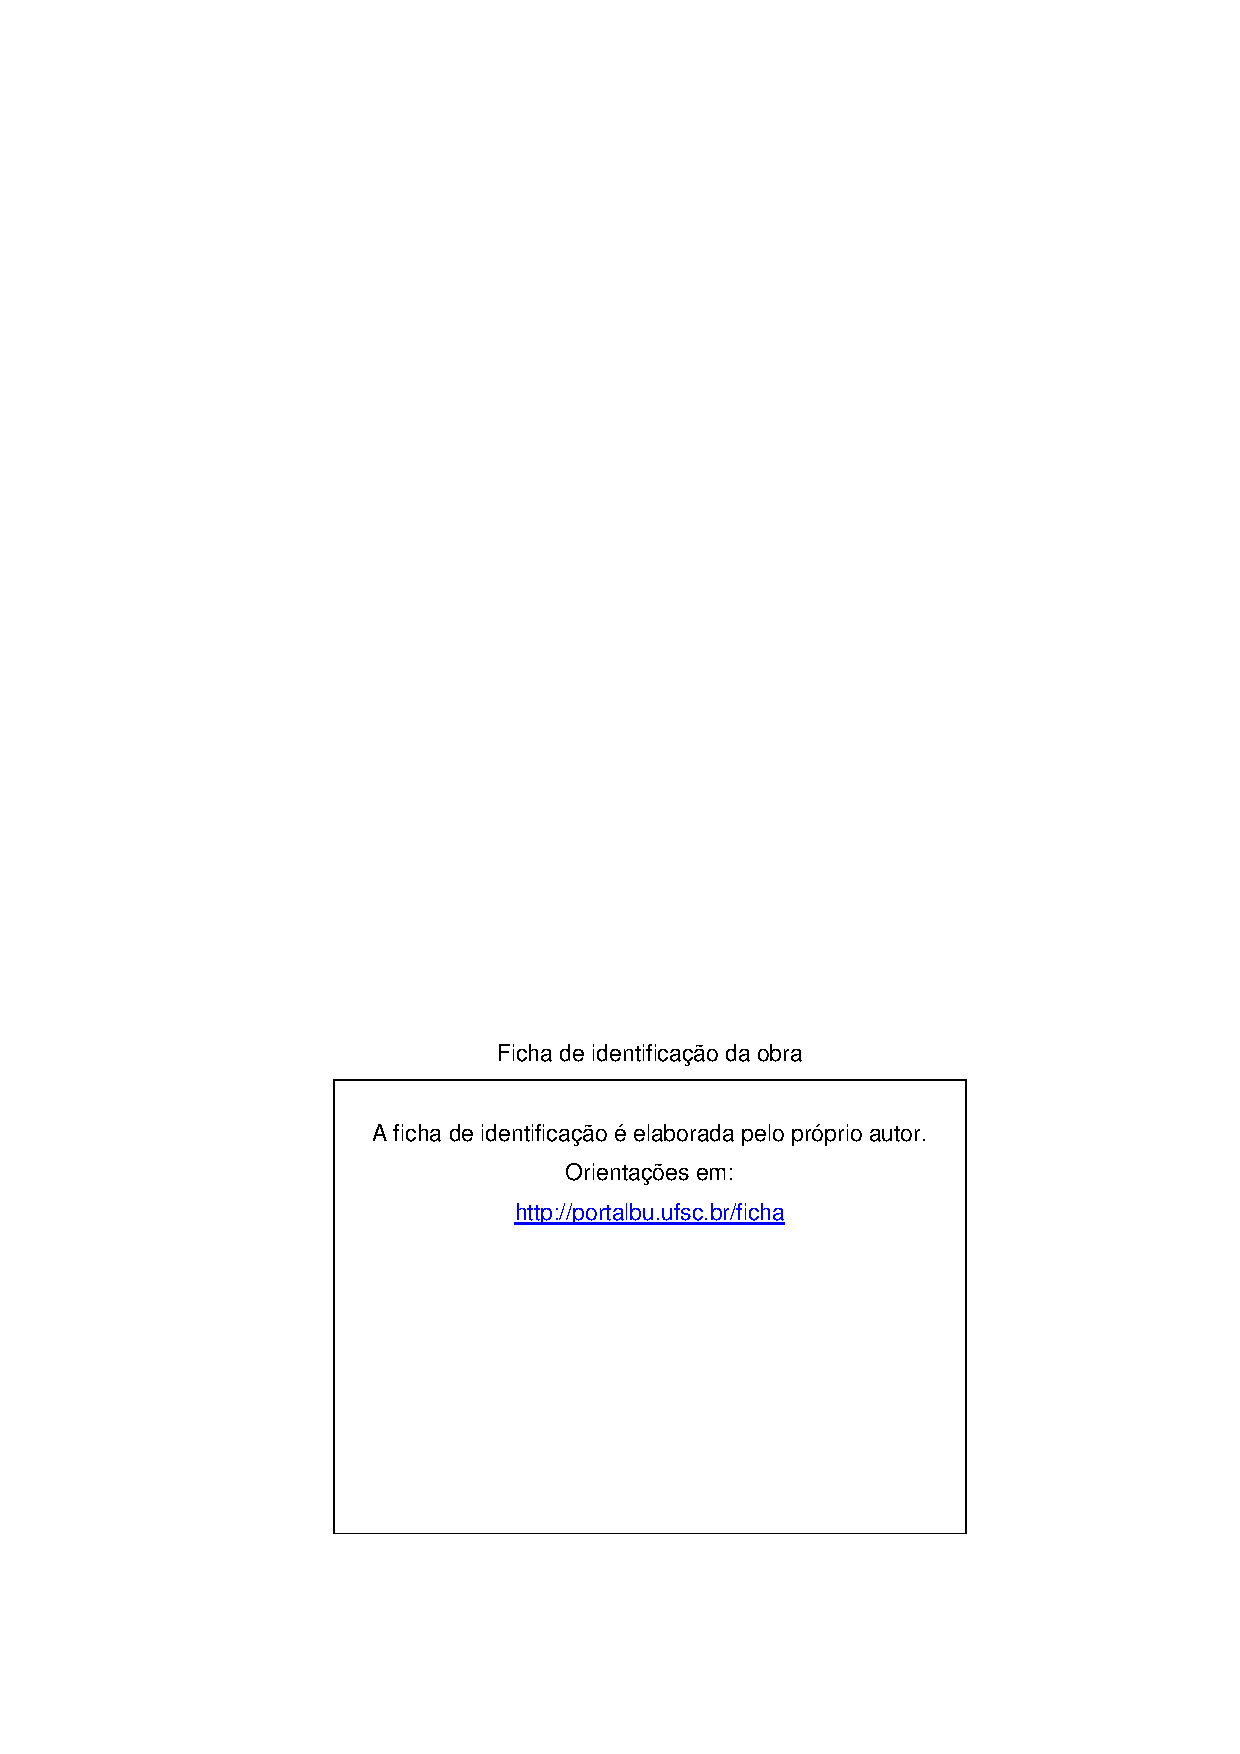
\includepdf{pre_textual/ficha_catalografica.pdf}
% \end{fichacatalografica}

% % Inserir folha de aprovação
% \begin{folhadeaprovacao}
% 	\OnehalfSpacing
% 	\centering
% 	\imprimirautor\\%
% 	\vspace{24pt}		
% 	\textbf{\imprimirtitulo}%
% 	\ifnotempty{\imprimirsubtitulo}{:~\imprimirsubtitulo}\\%
% 	%		\vspace*{31.5pt}%3\baselineskip
% 	\vspace*{\baselineskip}
% 	%\begin{minipage}{\textwidth}
% 	Este Trabalho de Conclusão de Curso foi julgao adequado para obtenção do Título de ``\imprimirformacao'' e aprovado em sua forma final pelo Curso de Graduação em Engenharia de Controle e Automação.\\
% 	\vspace{12pt}
% 	\imprimirlocal, \imprimirdia~de~\imprimirmes~de~\imprimirano.\\
	
% 	\vspace*{18pt}
% 	\textbf{Banca Examinadora:}\\
	
% 	\vspace*{24pt}
% 	\assinatura{\OnehalfSpacing \imprimirbancanomea}
% 	\vspace{6pt}
% 	\imprimirbancainsta\\
	
% 	\vspace*{24pt}
% 	\assinatura{\OnehalfSpacing \imprimirbancanomeb}
% 	\vspace{6pt}
% 	\imprimirbancainstb\\
	
% 	\vspace*{24pt}
% 	\assinatura{\OnehalfSpacing \imprimirbancanomec}
% 	\vspace{6pt}
% 	\imprimirbancainstc\\
	
% \end{folhadeaprovacao}

% Dedicatória
\ifnotempty{\imprimirdedicatoriatcc}{
\begin{dedicatoria}
	\vspace*{\fill}
	\noindent
	\begin{adjustwidth*}{}{7.5cm} 
		\textit{\imprimirdedicatoriatcc}
	\end{adjustwidth*}
\end{dedicatoria}
}

% Agradecimentos
\ifnotempty{\imprimiragradecimentostcc}{
\begin{agradecimentos}
	\imprimiragradecimentostcc
\end{agradecimentos}
}

% EPÍGRAFE
%\IFNOTEMPTY{\IMPRIMIREPIGRAFETCC}{
%\BEGIN{EPIGRAFE}
	%\VSPACE*{\FILL}
        %\NOINDENT
	%\BEGIN{ADJUSTWIDTH*}{}{7.5CM}
	       %\TEXTIT{\IMPRIMIREPIGRAFETCC}
        %\END{ADJUSTWIDTH*}
%\END{EPIGRAFE}
%}


% Resumo
\setlength{\absparsep}{18pt} % ajusta o espaçamento dos parágrafos do resumo
\begin{resumo}
	\SingleSpacing
	\imprimirresumotcc
	
	\textbf{Palavras-chave}: \imprimirpalavraschave
\end{resumo}

% Abstract
\begin{resumo}[Abstract]
	\SingleSpacing
	\imprimirabstracttcc
		
	\textbf{Keywords}: \imprimirkeywords
\end{resumo}

% Inserir publicações. Caso não deseje informa comentar todo esse bloco de código
% \begin{folhadeaprovacao}

% \cleardoublepage
% \begin{center}
%   {\textbf{PUBLICAÇÕES \textcolor{red}{Está página é opcional}}}
% \end{center}
% Esta dissertação é baseada no(s) artigo(s) científico(s) publicado(s) na(s) seguinte(s) revista(s):
% \vspace{1em}
% \begin{itemize}
%   \item SANTIAGO, Wagner Carvalho; KROETZ, Henrique Machado; SANTOS, Sérgio Hampshire de C.; STUCCHI, Fernando Rebouças; BECK, André Teófilo. Reliability-based calibration of main Brazilian structural design codes. \textbf{Latin American Journal of Solids and Structure}s, v. 17, e245, fev. 2020.
% \end{itemize}
% \cleardoublepage
	
% \end{folhadeaprovacao}

{%hidelinks
	\hypersetup{hidelinks}
	
	% inserir lista de figuras
	\pdfbookmark[0]{\listfigurename}{lof}
	\listoffigures*
	\cleardoublepage
	
	% inserir lista de quadros
	\ifnotempty{\verificaquadros}{
		\pdfbookmark[0]{\listofquadrosname}{loq}
		\listofquadros*
		\cleardoublepage
	}
	
	% inserir lista de tabelas
	\pdfbookmark[0]{\listtablename}{lot}
	\listoftables*
	\cleardoublepage
	
	% inserir lista de abreviaturas e siglas (devem ser declarados no preambulo)
	\ifnotempty{\verificasiglas}{
	\imprimirlistadesiglas
	}
	
	% inserir lista de símbolos (devem ser declarados no preambulo)
	\ifnotempty{\verificasimbolos}{
	\imprimirlistadesimbolos
	}

	% inserir o sumario
	\pdfbookmark[0]{\contentsname}{toc}
	\tableofcontents*
	\cleardoublepage
	
}%hidelinks